\documentclass[a4paper,12pt]{scrreprt}
    %% Used for changing geometry of the page
    %% Cover page text cannot overlay cover sketching/style 
    %% https://ctan.org/pkg/geometry?lang=en
\usepackage{geometry}
    %% Changes language of some packages protocols
    %% e.g., when captioning images: Figure 1. -> Figura 1.
    %% https://ctan.org/pkg/babel?lang=en
\usepackage[portuguese]{babel}
    %% Used for special fonts
    %% Cannot be compiled with pdflatex
    %% https://ctan.org/pkg/fontspec?lang=en
\usepackage{fontspec}
    %% Arial FONT
    \setmainfont{Arial}

    %% More colors and color options
    %% https://ctan.org/pkg/xcolor?lang=en
    %% https://ctan.org/pkg/colortbl?lang=en
\usepackage{xcolor,colortbl}
    %% More tabular options, like dashed/dotted lines
    %% https://ctan.org/pkg/arydshln?lang=en
\usepackage{arydshln}
    %% List of acronyms
    %% https://ctan.org/pkg/nomencl?lang=en
\usepackage[intoc]{nomencl}
    %% Must be called to init nomencl environment  
    \makenomenclature
    %% More images options/settings
    %% https://ctan.org/pkg/graphicx?lang=en
\usepackage{graphics}
    %% Defining subdirectories to image path enviornment
    %% \graphicspath{{sub1}{sub2}...{subN}}
    \graphicspath{{images}}
    
    %% used to handle cross-referencing commands in LaTeX to produce hypertext links in the document
    %% https://ctan.org/pkg/hyperref?lang=en
\usepackage{hyperref}
    %% math environments
    %% https://ctan.org/pkg/amsmath?lang=en

    %% settings
    \hypersetup{
        colorlinks,
        citecolor=black,
        filecolor=black,
        linkcolor=black,
        urlcolor=black
    }

\usepackage{amsmath}
    %% Defining backgrouns, used to make the cover
    %% https://ctan.org/pkg/background?lang=en
\usepackage[some]{background}
    %% Used to make drawings or complex graphics
    %% http://pgf.sourceforge.net/pgf_CVS.pdf
\usepackage{tikz}
    %% Tikz library to point operations ((x1,y1) + (x2,y2))
    \usetikzlibrary{calc}

%% Defining sfdefault font and default font for document
\renewcommand{\familydefault}{\sfdefault}


%% Costume made cover 
%% From there you can use \makecover command to build the cover
%% Blue cover color
\definecolor{titlepagecolor}{RGB}{54,95,145}

%==========================================================================
% COLORED BAR ON THE LEFT SIDE
%==========================================================================

\backgroundsetup{
    scale=1, 
    angle=0, 
    opacity=1,
    contents={
        \begin{tikzpicture}[remember picture,overlay]
            \fill[titlepagecolor] (-11,15) rectangle (-5,-20);
            \node[color=white] at (-7,-12) {\bfseries {\fontsize{120}{60} \textsf{L}}};
            \node[titlepagecolor] at (-3.5,-12) {\bfseries {\fontsize{120}{60} \textsf{I3}}};
            \node[color=titlepagecolor] at ($(current page.south west) + (5.8,4)$) {\bfseries {\fontsize{120}{60} \textsf{4}}};
        \end{tikzpicture}
    }
}

%==========================================================================
% TITLE PAGE INFO
%==========================================================================

%% Changes values in this field to show information in the cover and back cover about your team/project


%% TITLE
\title{Trabalho Prático LI3  \newline \newline
Fase 1  \newline\newline Grupo 35}



%% AUTHORS
\author{
     \hspace{0.25cm} 
  \newline
  Flávio David Rodrigues Sousa $($A100715$)$
  \newline
  André Miguel Alves de Carvalho $($A100818$)$
     \hspace{1.15cm}
  \newline
  Sandro José Rodrigues Coelho
     \hspace{0.15cm} $($A105672$)$
}

%% Date

\date{\today}

%% Course
\newcommand{\Course}{Licenciatura em Engenharia Informática}

%% Department
\newcommand{\Department}{Escola de Engenharia}

%% UniName
\newcommand{\UniName}{Universidade do Minho}

%% UniPic
\newcommand{\UniPic}{
\includegraphics[scale=0.09]{images/uminho.png}}

%% University 
\newcommand{\University}{
    \begin{flushleft}
        \UniPic
    \end{flushleft}
    \textcolor{gray}{\small\textbf{\textsf{\UniName}}}\par
    \textcolor{gray!80!white}{\small{\textsf{\Department}}}\par
    \textcolor{gray!70!white}{\small{\textsf{\Course}}}
}

%% UC
\newcommand{\UC}{
    \begin{flushleft}
        \par\textcolor{titlepagecolor}{  \LARGE\textbf{\textsf{Unidade Curricular de \\ Redes de Computadores}}}
    \end{flushleft}
}

%% School Year
\newcommand{\SchoolYear}{
    \small{\textsf{Ano Letivo de 2023/2024}}}


%% Define new command to show title, author and date
\makeatletter
\let\Title\@title
\let\Author\@author
\let\Date\@date
\makeatother





%% MAKETEMPLATE
\newcommand{\makecover}{

%==========================================================================
% BEGIN COVER PAGE 
%==========================================================================

%% Removes page number on footer
\thispagestyle{empty}

%% No indentation 
\setlength{\parindent}{0em}

%% Put Background defined on \backgroundsetup, in this page
\BgThispage

%% Changing geometry to prevent overlay with text
%% At the end of back cover, geometry is default with \restoregeometry
\newgeometry{top=5cm,left=6cm,right=3cm,bottom=2cm}

%% builds university info defined previously
\University
\vspace{1cm}
%% builds curricular unity info defined previously
\UC
%% builds school year info defined previously
\SchoolYear

\vspace*{5cm}
%% bigger space (i think its the default one) between paragraphs 
\setlength{\parskip}{1em}

%% builds title info defined previously
\par\textbf{\textsf{\huge\Title}}
\vspace{1cm}
%% builds author(s) info defined previously
\par\Author

\vspace{0.5cm}

%% builds date info defined previously
\par\Date
\restoregeometry
\pagebreak

%==========================================================================
% END COVER PAGE 
%==========================================================================

%==========================================================================
% BEGIN BACK COVER PAGE 
%==========================================================================

%% Removes page number on footer
\thispagestyle{empty}

% Changing look of lines in tabular environment 
% Dashed -> dotted 
%% length of dashes
\setlength\dashlinedash{0.3pt}
%% space between dashes
\setlength\dashlinegap{1.5pt}
%% width of dashes
\setlength\arrayrulewidth{1.1pt}


%% This values can be changed in the preamble




\pagebreak
%==========================================================================
% END BACK COVER PAGE 
%==========================================================================
}


%==========================================================================
% DOCUMENT
%==========================================================================

\begin{document}

\pagenumbering{gobble}

% builds the cover
\makecover

%% smaller footer and header size
\newgeometry{top=3cm,left=3cm,right=3cm,bottom=4cm}



%==========================================================================
% BEGIN INDEXES PAGES
%==========================================================================

%% Changes table of content name
%% Portuguese babel default : "Conteúdo"
%% Personally I prefer "índice"
\renewcommand{\contentsname}{Índice}

\tableofcontents

\pagebreak


\pagebreak

\pagebreak

%==========================================================================
% END INDEXES PAGES 
%==========================================================================


%==========================================================================
% BEGIN INTRODUCTION
%==========================================================================

%% Starting page numbering here
\pagenumbering{arabic}


    
    

%==========================================================================
% END INTRODUCTION
%==========================================================================

%==========================================================================
% BEGIN PRIMEIRA FASE DO RELATÓRIO
%==========================================================================

\chapter{Introdução}

Este projeto que se encontra em desenvolvimento ao longo do ano letivo 2023/24 na unidade curricular de LI3 (Laboratórios de Informática III). Esta tem como objetivo refinar os conhecimentos adquiridos da linguagem C e de aprimorar o mesmo conhecimento sobre Engenharia de Software, nomeadamente, conhecimento envolvendo modularidade, encapsulamento, validação funcional, estruturas dinâmicas de dados e medição de desempenho de um programa.

O projeto em questão encontra-se dividido em duas fases, sendo este relatório destinado à primeira fase do trabalho prático, referindo-se a \textit{parsing} de dados, o modo batch e o desenvolvimento de no mínimo sessenta porcento das \textit{queries}, ficando no critério dos alunos sobre quais \textit{queries} querem implementar para esta fase. 

Estas \textit{queries} serão executadas por comandos pré-definidos pelos docentes da unidade curricular, de modo a poder testar todos os aspetos do código presente, armazenando por fim os resultados de cada comando em ficheiros de texto. 

Por fim, estes ficheiros são testados na plataforma online da unidade curricular (\href{https://li3.di.uminho.pt}{Plataforma de Teste}), de modo a descobrir se existe algum erro com as \textit{queries}, ou com o modo com que entregam os seus outputs.

\chapter{Desenvolvimento}

Para realizar o trabalho de forma mais eficaz, decidimos dividir o código, pois seria mais fácil de controlar o que estaria a ser realizado sobre cada parte do projeto, sendo a realização total do pedaço de código, resolução de \textit{memory leaks} ou até mesmo renovação de código de modo a que o mesmo seja mais eficaz.

Com essa ideia em mente, foi possível dividir o desenvolvimento do \textit{parser} para um aluno em particular enquanto ou outros dois alunos realizavam as \textit{queries} escolhidas.

\begin{figure}[htb!]
        \centering
        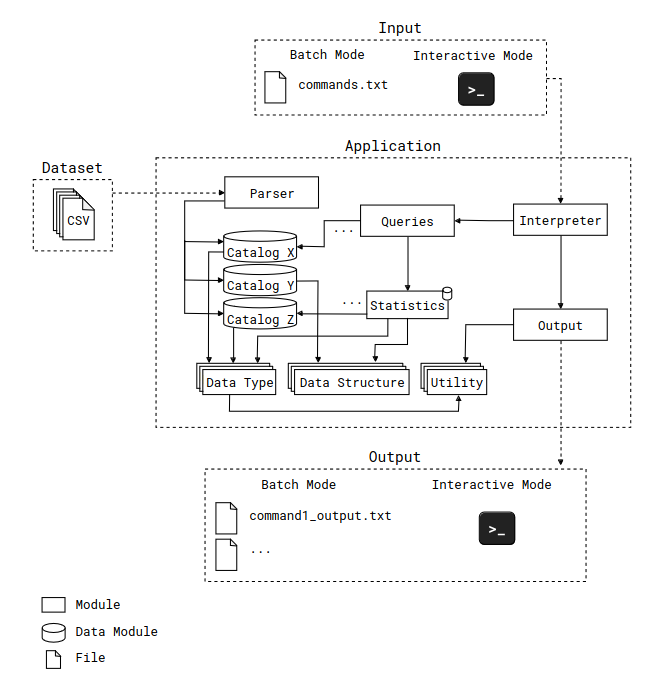
\includegraphics[width =0.7\textwidth]{images/ArquiteturaReferencia.png}
        \caption{Arquitetura de referência entregue pelos docentes}
        \label{fig:my_label}
    \end{figure}

Após abordarmos a fase de planeamento do trabalho, começamos com a base do mesmo, verificando a integridade de todos os dados que seriam manipulados pelo programa, de modo a que seja possível validar cada documento.

Com isso, foi implementado o parser, sendo a parte mais importante do programa, permitindo a análise e entendimento dos dados fornecidos. Esta etapa envolveu a criação eficiente de um algoritmo para processar e interpretar todos os dados que o atravessam, garantindo assim uma transição rápida e eficaz.

Em seguida, foi necessário criar as funções responsáveis por manipular as \textit{queries} criadas, de modo a que fosse possível obter os resultados necessários para os comandos fornecidos. Durante este processo, percebemos a necessidade de criar estruturas adicionais para otimizar certas \textit{queries}. Neste caso, foram usadas árvores para certas \textit{queries}.

Por fim, incorporamos um modo de execução \textit{batch}, facilitando a experiência dos utilizadores. Esta é a etapa final, conseguindo trazer todo o potencial existente das \textit{queries} para o programa.

\section{Queries}

A implementação das \textit{queries} foi uma parte do projeto que necessitou de atenção extra, devido à complexidade que a maioria delas tinha, sendo essenciais para o funcionamento do programa, estas representam os pedidos dos utilizadores, obtendo assim as informações pedidas. Com isto, foi possível verificar a importância dos pedidos, assim como a importância da estratégia usada para que o programa pudesse ser resolvida da forma mais eficaz possível, fornecendo resultados coerentes e rigorosos.

\subsection{Query 1}

A primeira \textit{query} consiste em \textit{"Listar o resumo de um utilizador, voo, ou reserva, consoante o identificador recebido por argumento."}, este entrega as informações destinadas ao argumento entregue pelo utilizador, dependendo do identificador recebido. 

Se o identificador começar com \textit{"0000"}, a função irá trata-lo como um voo, entregando as informações relacionadas com ele, tal como a companhia, avião, origem, destino, hora de partida estimada, hora de chegada estimada, número de passageiros e o tempo de atraso.

Se o identificador começar com \textit{"Book"}, a função irá trata-lo como uma reserva, entregado as suas informações, tal como ID do hotel, nome do hotel, quantidade das estrelas do hotel, data de começo, data de fim da reserva, se a reserva inclui pequeno-almoço, quantidade de noites passadas e preço total da mesma.

Se o identificador não for nenhum dos anteriores, será tratado como um utilizador, entregando assim as informações referentes ao mesmo, tal como, nome, sexo, idade, código do país, passaporte, numero de voos, numero de reservas e total gasto.

Por fim, a função verifica se \textit{type} da função, dependendo do seu valor, as funções serão escritas no formato correto para o ficheiro de saída. Além disso, é alocada memória sempre que é armazenada alguma informação, logo, é necessário libertar essa memória de modo a não haver \textit{memory leaks} no programa.

\subsection{Query 2}

A segunda \textit{query}, consiste em \textit{Listar os voos ou reservas de um utilizador, se o segundo argumento for flights ou reservations,
respetivamente, ordenados por data (da mais recente para a mais antiga). Caso não seja fornecido
um segundo argumento, apresentar voos e reservas, juntamente com o tipo.}

Esta função utiliza funções auxiliares para criar e organizar as listas de voos e reservas, imprimindo os seus resultados no formato desejado para o ficheiro de saída.

Com as funções auxiliares criadas, é possível identificar os voos e reservas que se encontram associados ao utilizador, permitindo assim a criação de árvores ordenadas através da data e do \textit{ID}.

Com isto, são usadas outras funções de modo a organizar as árvores por data, realizando a comparação entre as mesmas.

\subsection{Query 3}

A terceira \textit{query}, consiste em \textit{Apresentar a classificação média de um hotel, a partir do seu identificador}.

A função percorre as reservas, e verifica se pertencem ao hotel desejado, se assim for, soma as classificações e a quantidade de classificações, criando assim a média da mesma no fim.

Caso não haja nenhuma reserva para o hotel, é escrita uma linha vazia no ficheiro de saída, caso contrário, formata a média e escreve-a no ficheiro de saída.

\subsection{Query 4}

A quarta \textit{query}, consiste em \textit{Listar as reservas de um hotel, ordenadas por data de início (da mais recente para a mais antiga). Caso duas reservas tenham a mesma data, deve ser usado o identificador da reserva como critério de desempate (de forma crescente).}.

A função utiliza uma função auxiliar de modo a construir uma árvore capaz de armazenar as reservas associadas a um certo hotel. 

As várias funções auxiliares presentes, desempenham os seus papéis para a funcionalidade da árvore, tal como a criação, manipulação, libertação, contagem e ordenação das árvores criadas.

No fim, é revisto todas as reservas presentes, identificando aquelas associadas ao hotel que se encontra escolhido pelo utilizador, ordenando-as assim por data e \textit{ID}, imprimindo as informações no formato desejado.

\subsection{Query 5}

\subsection{Query 9}

A nona \textit{query}, consiste em \textit{Listar todos os utilizadores cujo nome começa com o prefixo passado por argumento, ordenados por nome de forma crescente}. Caso ambos nomes sejam iguais, é organizado através do \textit{ID} do utilizador.

A função compara ambos nomes de modo a organizar ambos através de ordenação sensível a cada idioma.
Durante a execução, a função compara os nomes através do prefixo de cada nome, se ambos prefixos forem iguais, é verificada a letra seguinte, até achar uma letra que seja diferente da que está a ser comparada, ordenando assim os nomes, caso contrário, se os nomes forem iguais, é necessário comparar os \textit{IDs} dos utilizadores e ordenar os nomes através deles.

Por fim, os resultados são ordenados usando a função \textit{qsort} e a função criada para comparação personalizada, formatando e escrevendo os resultados no ficheiro de saída.




%==========================================================================
% END PRIMEIRA FASE DO RELATÓRIO
%==========================================================================



%==========================================================================
% BEGIN CONCLUSÕES DE TRABALHO FUTURO
%==========================================================================

    

%==========================================================================
% END CONCLUSÕES DE TRABALHO FUTURO
%==========================================================================



\end{document}